\chapter{Bitcoin}
\label{chapter:bitcoin}
Bitcoin (BTC) is a decentralized digital currency without a central bank or single administrator.
The original paper \cite{bitcoin_2008} and the first implementation of Bitcoin were published respectively in November \num{2008} and January \num{2009} by an unknown person or group of people using the name of Satoshi Nakamoto \cite{bitcoin_website}.
Since its release, Bitcoin has gained popularity and attention of the media, especially between the end of \num{2017} and the beginning of \num{2018} \cite{bbc_2018, telegraph_2018, ilsole24ore_2018}.
Nowadays, Bitcoin is the most used and valuable cryptocurrency available on the market, with a price of over \SI{8000}{\$ \per BTC} and a market cup of about \SI{141000000000}{\$} \cite{bitcoin_usage_study_2017, stats_coinmarketcap, stats_coinranking, stats_cryptocompare, stats_coincheckup, stats_moonstats}.
Bitcoin can be used for both online and in-shop payments, fast and low-cost money transfer, and pseudonymous money spending.

\bigskip
Bitcoin is a complex technology that takes advantage of modern cryptography and distributed algorithms to solve the complex Byzantine Consensus problem \cite{byzantin_generals_1982}.
This section covers the main building blocks and concepts and gives an overview of the overall working of Bitcoin.

\section{Blockchain}
The blockchain is a decentralized, distributed, public digital ledger that records Bitcoin transactions.
It is implemented as a chain of blocks, connected to each other using linked timestamping \cite{bitcoin_book_narayanan_2016, hash_function_wikipedia}:
each block stores the cryptographic hash of the previous one (\cref{fig:blockchain}).
This technique guarantees that the transactions stored in the ledger can not be changed easily, since a single modification would break the hashes of each following block in the chain.
The first block is called ``genesis'' and it is hard-coded in the software implementation.

Nodes that participate in the Bitcoin protocol run a consensus algorithm to agree on the order of blocks in the ledger:
in particular, it is enough to agree on the last block in the chain, thanks to the guarantees given by linked timestamping.
The blockchain is stored in each computer that participates in the consensus:
the geographical distribution of nodes around the world and the decentralization of the protocol make attacks that tries to change the history of transactions stored in the ledger very difficult or nearly impossible to achieve.

\begin{figure}[h]
	\centering
	\vspace*{0.25cm}
	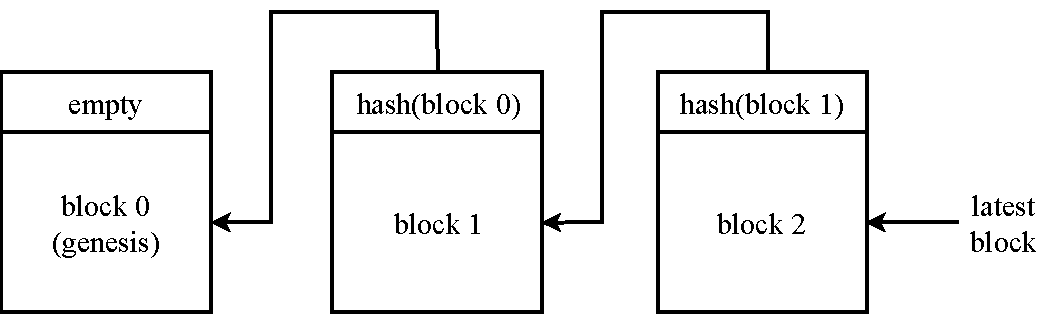
\includegraphics[scale=0.7]{figures/blockchain}
	\vspace*{0.25cm}
	\caption{
		Schematic representation of a blockchain.
		A blockchain is a list of blocks, connected to each other with an hash pointer.
		Each block contains a set of transactions.
	}
	\label{fig:blockchain}
\end{figure}

\section{Blocks}
Each block contains and confirms a number of transactions up to about \num{3000}.
By design, a new block is generated and appended to the blockchain every \num{10} minutes on average \cite{bitcoin_2008}.
Bitcoin blocks are distributed using a peer-to-peer protocol, which is explained in \cref{chapter:protocol}.

The transactions inside each block are organized as a Merkle tree \cite{merkle_tree_1980}, a special binary tree with hash pointers (\cref{fig:merkle}).
The items in the tree are grouped in pairs and the hash of each of them is stored in the parent node.
The parent nodes are then grouped in other pairs and their hashed are stored in their parents:
this construction is repeated recursively until a single root node is created.
In the specific case of Bitcoin, each item in the tree represents a single transaction.

\begin{figure}[h]
	\centering
	\vspace*{0.1cm}
	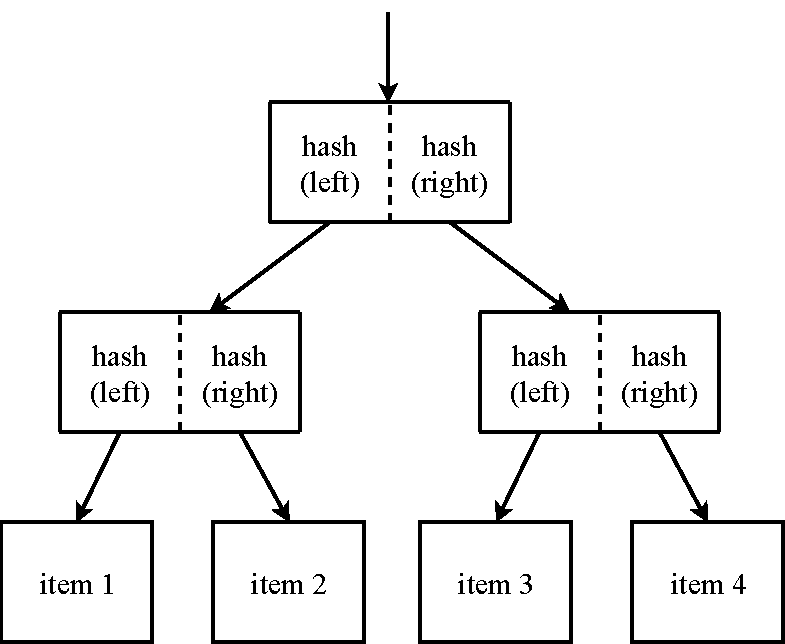
\includegraphics[scale=0.7]{figures/merkle}
	\vspace*{0.25cm}
	\caption{Schematic representation of a Merkle tree with \num{4} items.}
	\label{fig:merkle}
\end{figure}

The main advantage of using a Merkle tree is that the hash of the root uniquely identifies a specific set of transactions.
In fact, a change of a single item would modify the hashes of all ancestor nodes in the tree, thanks to the properties of the cryptographic hash functions.
This allows to divide a Bitcoin block in \num{2} parts - a header and a body - and distribute them independently of each other \cite{bitcoin_reference}.
The header contains only the hash of the Merkle tree root, the hash of the previous block in the blockchain and a couple of additional information such as protocol version and timestamp of creation.
The body stores the set the transactions as a serialized representation of the Merkle tree.

The second advantage of a Merkle tree is that transaction lookups in a block take $\mathcal{O}(n\log n)$ time, where $n$ is the number of transactions stored in the block.

\section{Transactions}
Transactions are used to spend bitcoins, i.e. move bitcoins between different addresses (see \cref{sec:addresses}).
Transactions in Bitcoin are not as simple as a tuple of \texttt{\textlangle sender, amount, receiver\textrangle}.
They are expressed as a small script, written in a custom, stateless and non-Turing-complete language.
Transactions can have many inputs and many outputs, offer a transaction fee as incentive to be processed faster (see \cref{sec:mining}) or even define a kind of contract between parties (for example, some money ``spent'' in the transaction might be redeemable only on certain conditions).

For the sake of this thesis, we do not need to go into all details of Bitcoin transactions, which can be found in the Bitcoin Developer Guide \cite{bitcoin_guide}.
It is only important to outline that:
\begin{itemize}
	\item the history of all transactions is stored in the blockchain and allows to deterministically compute balances and validate new transactions (new transactions can only spend bitcoins that are available in an address, i.e. not already spent);
	\item transactions are valid only if signed with the private key of the owner of the address, so that nobody can steal bitcoins from third parties addresses without permission.
\end{itemize}

\section{Addresses}
\label{sec:addresses}
A Bitcoin address corresponds to a pair of public and private key: the hash of the public key is the actual Bitcoin address, while the private key is needed to make payments using the bitcoins stored in the address.
Each address can store some bitcoins, which are the result of some transaction stored in the blockchain.
The owner of the private key associated to the address is able to create valid transactions to move the stored bitcoins to other addresses, or to create a contract.

A Bitcoin address can be compared to the concept a bank account:
it stores an amount of money (bitcoins in this case) and it is the only information required to make a payment to someone;
in addition, only the owner is able to spend the money contained in the account.
In contrast to traditional bank accounts, Bitcoin developers suggest to use each address only for a single transactions to preserve the privacy of the owner \cite{bitcoin_guide}:
since all transactions are publicly stored in the blockchain, it is trivial to trace all transactions involving a specific address.

\section{Wallets}
A wallet is a convenient way to manage Bitcoin addresses.
Bitcoin wallets create public keys (i.e. addresses) where to receive bitcoins and use the corresponding private keys to spend the bitcoins in the addresses.
They can simultaneously manage multiple addresses and provide a nice user interface to facilitate different tasks, such as buying something in a shop or make an online payment.
A wallet also solves the problem or ``rotating'' addresses at each transaction in order to make the user more difficult to track, without need of human intervention or understanding of all exact operations performed from the waller owner.

Wallets can be either a software or a physical device.
Software wallets are usually easier to use, since they can simply use the available internet connection to interact with the peer-to-peer network to get information from the blockchain and broadcast new transactions.
On the other hand, software wallets more vulnerable to attacks, since an attacker only needs to compromise the user's device running the software to steal the private keys stored in the wallet and take control of the bitcoins stored in the corresponding addresses.
Hardware wallets are physical devices able to manage Bitcoin addresses and store the private keys securely in a dedicated hardware module.

\section{Forks}
A fork is a bifurcation of the blockchain:
it happens when \num{2} or more different blocks have the same parent block, as shown in \cref{fig:forks}.
Blocks in different branches in the blockchain may contain different or even contrasting transactions and create inconsistencies in the global state, since different nodes may decide to follow different forks.
To solve this problem, Bitcoin introduces a resolution rule for forks:
correct Bitcoin nodes should follow the longest chain, i.e. the chain whose last block has the higher number of preceding blocks.

\begin{figure}[h]
	\centering
	\vspace*{0.25cm}
	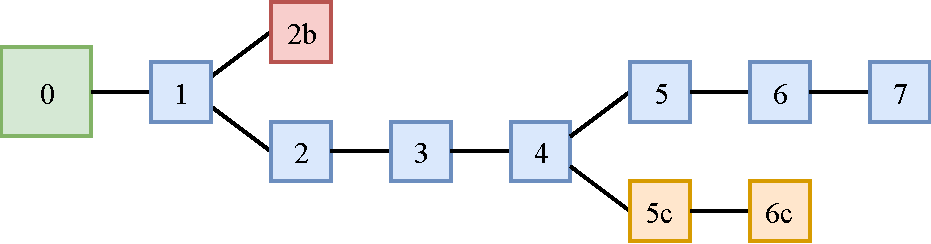
\includegraphics[scale=0.8]{figures/forks}
	\vspace*{0.25cm}
	\caption{
		Schematic representation of a blockchain with \num{3} branches.
		The red block \texttt{2b} and the yellow blocks \texttt{5c} and \texttt{6c} are forks of the main chain that originate respectively at blocks \texttt{1} and \texttt{4}.
		Blue blocks are on the longest chain, since block \texttt{7} is the one with the highest number of preceding blocks.
		The green block represents represents the ``genesis''.
	}
	\label{fig:forks}
\end{figure}

Forks are probably the biggest problem in Bitcoin, since they allow an attacker to try to spend the money twice by creating two contrasting transactions that get stored in blocks published on different branches of the blockchain.
We will cover the ``double-spend'' attack in greater detail in \cref{chapter:attacks}.

\section{Mining \& Proof of Work}
\label{sec:mining}
The usage of modern cryptography in Bitcoin addresses and transactions guarantees that only the owner of some money can actually spend it (at least until the private key associated to the address is carefully protected).
Also, since all transactions are recorded and stored in the blockchain, the blockchain uses cryptographic hashes to detect tampering and it is replicated around many computer and devices around the world, it is very difficult or even impossible to remove old transactions from the past (i.e. revert payments).
However, there is so far no mechanism that prevents an attacker to create a big number of forks by forging new blocks.

Bitcoin uses \ac{PoW} \cite{pow_2002} to reduce the feasibility of such an attack.
It requires to solve a cryptographic puzzle and include the its solution to make a block valid.
The difficulty of the puzzle is agreed by the network depending on the total computational power available.
The puzzle consists in finding a nonce to include in the block such that the cryptographic hash of the serialized block is less than a target number, i.e. it starts with a certain number of zeros.
Thanks to the properties of cryptographic hash functions, the only way to solve the puzzle is a brute-force approach, which requires time and resources (in terms of both computation power and energy).
This mechanism prevents an attacker to forge too many blocks, since it would require too many resources and time.
